\documentclass{article}
\usepackage[T1]{fontenc}
\usepackage{lmodern}
\usepackage{graphicx}
\usepackage{amsmath,amssymb}
\usepackage[a4paper,margin=2cm]{geometry}
\usepackage[absolute,overlay]{textpos}
\setlength{\TPHorizModule}{1mm}
\setlength{\TPVertModule}{1mm}
\usepackage[indonesian]{babel}
\usepackage{hyperref}
\setlength{\emergencystretch}{2em}
% unit: Halaman 5

\begin{document}

% === Halaman 5 (llm) ===

\begin{itemize}
  \item Pada bulan Oktober 2000, \textit{NIST} mengumumkan untuk memilih Rijndael (dibaca: Rhine-doll)
  \item Pada bulan November 2001, Rijndael ditetapkan sebagai AES
\end{itemize}

\vspace{50mm}

\begin{itemize}
  \item Diharapkan Rijndael menjadi standard kriptografi yang dominan paling sedikit selama 10 tahun.
\end{itemize}

% deskripsi: Foto dua orang pria di depan papan bertuliskan AES (Advanced Encryption Standard)
% bbox normalisasi: [0.2710, 0.3380, 0.6080, 0.7630]
\begin{textblock*}{70.77mm}(56.91mm,100.39mm)
\noindent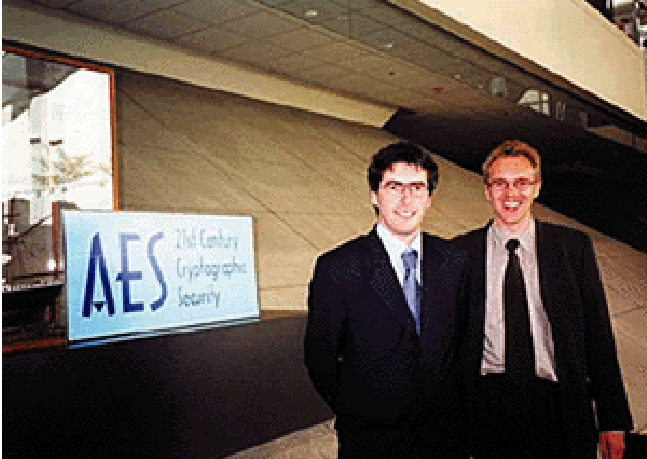
\includegraphics[width=70.77mm,height=126.22mm]{../../images/llm/page_005_img_01.png}%
\end{textblock*}

\end{document}
